% Options for packages loaded elsewhere
% Options for packages loaded elsewhere
\PassOptionsToPackage{unicode}{hyperref}
\PassOptionsToPackage{hyphens}{url}
\PassOptionsToPackage{dvipsnames,svgnames,x11names}{xcolor}
%
\documentclass[
  spanish,
  letterpaper,
  DIV=11,
  numbers=noendperiod,
  oneside]{scrartcl}
\usepackage{xcolor}
\usepackage[left=1in,marginparwidth=2.0666666666667in,textwidth=4.1333333333333in,marginparsep=0.3in]{geometry}
\usepackage{amsmath,amssymb}
\setcounter{secnumdepth}{-\maxdimen} % remove section numbering
\usepackage{iftex}
\ifPDFTeX
  \usepackage[T1]{fontenc}
  \usepackage[utf8]{inputenc}
  \usepackage{textcomp} % provide euro and other symbols
\else % if luatex or xetex
  \usepackage{unicode-math} % this also loads fontspec
  \defaultfontfeatures{Scale=MatchLowercase}
  \defaultfontfeatures[\rmfamily]{Ligatures=TeX,Scale=1}
\fi
\usepackage{lmodern}
\ifPDFTeX\else
  % xetex/luatex font selection
\fi
% Use upquote if available, for straight quotes in verbatim environments
\IfFileExists{upquote.sty}{\usepackage{upquote}}{}
\IfFileExists{microtype.sty}{% use microtype if available
  \usepackage[]{microtype}
  \UseMicrotypeSet[protrusion]{basicmath} % disable protrusion for tt fonts
}{}
\makeatletter
\@ifundefined{KOMAClassName}{% if non-KOMA class
  \IfFileExists{parskip.sty}{%
    \usepackage{parskip}
  }{% else
    \setlength{\parindent}{0pt}
    \setlength{\parskip}{6pt plus 2pt minus 1pt}}
}{% if KOMA class
  \KOMAoptions{parskip=half}}
\makeatother
% Make \paragraph and \subparagraph free-standing
\makeatletter
\ifx\paragraph\undefined\else
  \let\oldparagraph\paragraph
  \renewcommand{\paragraph}{
    \@ifstar
      \xxxParagraphStar
      \xxxParagraphNoStar
  }
  \newcommand{\xxxParagraphStar}[1]{\oldparagraph*{#1}\mbox{}}
  \newcommand{\xxxParagraphNoStar}[1]{\oldparagraph{#1}\mbox{}}
\fi
\ifx\subparagraph\undefined\else
  \let\oldsubparagraph\subparagraph
  \renewcommand{\subparagraph}{
    \@ifstar
      \xxxSubParagraphStar
      \xxxSubParagraphNoStar
  }
  \newcommand{\xxxSubParagraphStar}[1]{\oldsubparagraph*{#1}\mbox{}}
  \newcommand{\xxxSubParagraphNoStar}[1]{\oldsubparagraph{#1}\mbox{}}
\fi
\makeatother


\usepackage{longtable,booktabs,array}
\usepackage{calc} % for calculating minipage widths
% Correct order of tables after \paragraph or \subparagraph
\usepackage{etoolbox}
\makeatletter
\patchcmd\longtable{\par}{\if@noskipsec\mbox{}\fi\par}{}{}
\makeatother
% Allow footnotes in longtable head/foot
\IfFileExists{footnotehyper.sty}{\usepackage{footnotehyper}}{\usepackage{footnote}}
\makesavenoteenv{longtable}
\usepackage{graphicx}
\makeatletter
\newsavebox\pandoc@box
\newcommand*\pandocbounded[1]{% scales image to fit in text height/width
  \sbox\pandoc@box{#1}%
  \Gscale@div\@tempa{\textheight}{\dimexpr\ht\pandoc@box+\dp\pandoc@box\relax}%
  \Gscale@div\@tempb{\linewidth}{\wd\pandoc@box}%
  \ifdim\@tempb\p@<\@tempa\p@\let\@tempa\@tempb\fi% select the smaller of both
  \ifdim\@tempa\p@<\p@\scalebox{\@tempa}{\usebox\pandoc@box}%
  \else\usebox{\pandoc@box}%
  \fi%
}
% Set default figure placement to htbp
\def\fps@figure{htbp}
\makeatother


% definitions for citeproc citations
\NewDocumentCommand\citeproctext{}{}
\NewDocumentCommand\citeproc{mm}{%
  \begingroup\def\citeproctext{#2}\cite{#1}\endgroup}
\makeatletter
 % allow citations to break across lines
 \let\@cite@ofmt\@firstofone
 % avoid brackets around text for \cite:
 \def\@biblabel#1{}
 \def\@cite#1#2{{#1\if@tempswa , #2\fi}}
\makeatother
\newlength{\cslhangindent}
\setlength{\cslhangindent}{1.5em}
\newlength{\csllabelwidth}
\setlength{\csllabelwidth}{3em}
\newenvironment{CSLReferences}[2] % #1 hanging-indent, #2 entry-spacing
 {\begin{list}{}{%
  \setlength{\itemindent}{0pt}
  \setlength{\leftmargin}{0pt}
  \setlength{\parsep}{0pt}
  % turn on hanging indent if param 1 is 1
  \ifodd #1
   \setlength{\leftmargin}{\cslhangindent}
   \setlength{\itemindent}{-1\cslhangindent}
  \fi
  % set entry spacing
  \setlength{\itemsep}{#2\baselineskip}}}
 {\end{list}}
\usepackage{calc}
\newcommand{\CSLBlock}[1]{\hfill\break\parbox[t]{\linewidth}{\strut\ignorespaces#1\strut}}
\newcommand{\CSLLeftMargin}[1]{\parbox[t]{\csllabelwidth}{\strut#1\strut}}
\newcommand{\CSLRightInline}[1]{\parbox[t]{\linewidth - \csllabelwidth}{\strut#1\strut}}
\newcommand{\CSLIndent}[1]{\hspace{\cslhangindent}#1}

\ifLuaTeX
\usepackage[bidi=basic]{babel}
\else
\usepackage[bidi=default]{babel}
\fi
% get rid of language-specific shorthands (see #6817):
\let\LanguageShortHands\languageshorthands
\def\languageshorthands#1{}


\setlength{\emergencystretch}{3em} % prevent overfull lines

\providecommand{\tightlist}{%
  \setlength{\itemsep}{0pt}\setlength{\parskip}{0pt}}



 


\KOMAoption{captions}{tableheading}
\makeatletter
\@ifpackageloaded{caption}{}{\usepackage{caption}}
\AtBeginDocument{%
\ifdefined\contentsname
  \renewcommand*\contentsname{Tabla de contenidos}
\else
  \newcommand\contentsname{Tabla de contenidos}
\fi
\ifdefined\listfigurename
  \renewcommand*\listfigurename{Listado de Figuras}
\else
  \newcommand\listfigurename{Listado de Figuras}
\fi
\ifdefined\listtablename
  \renewcommand*\listtablename{Listado de Tablas}
\else
  \newcommand\listtablename{Listado de Tablas}
\fi
\ifdefined\figurename
  \renewcommand*\figurename{Figura}
\else
  \newcommand\figurename{Figura}
\fi
\ifdefined\tablename
  \renewcommand*\tablename{Tabla}
\else
  \newcommand\tablename{Tabla}
\fi
}
\@ifpackageloaded{float}{}{\usepackage{float}}
\floatstyle{ruled}
\@ifundefined{c@chapter}{\newfloat{codelisting}{h}{lop}}{\newfloat{codelisting}{h}{lop}[chapter]}
\floatname{codelisting}{Listado}
\newcommand*\listoflistings{\listof{codelisting}{Listado de Listados}}
\makeatother
\makeatletter
\makeatother
\makeatletter
\@ifpackageloaded{caption}{}{\usepackage{caption}}
\@ifpackageloaded{subcaption}{}{\usepackage{subcaption}}
\makeatother
\makeatletter
\@ifpackageloaded{sidenotes}{}{\usepackage{sidenotes}}
\@ifpackageloaded{marginnote}{}{\usepackage{marginnote}}
\makeatother
\usepackage{bookmark}
\IfFileExists{xurl.sty}{\usepackage{xurl}}{} % add URL line breaks if available
\urlstyle{same}
\hypersetup{
  pdfauthor={Equipo EDUMER},
  pdflang={es},
  colorlinks=true,
  linkcolor={blue},
  filecolor={Maroon},
  citecolor={Blue},
  urlcolor={Blue},
  pdfcreator={LaTeX via pandoc}}


\author{Equipo EDUMER}
\date{}
\begin{document}


\pandocbounded{
\includegraphics[keepaspectratio]{images/coes.png}}

\pandocbounded{
\includegraphics[keepaspectratio]{images/LOGO-OCS.png}}

\pandocbounded{
\includegraphics[keepaspectratio]{images/qrcode.png}}

\section{\texorpdfstring{\textbf{Cohesión social y
migración}:}{Cohesión social y migración:}}\label{cohesiuxf3n-social-y-migraciuxf3n}

\subsection{\texorpdfstring{\textbf{Una década de cambios y
desafíos}}{Una década de cambios y desafíos}}\label{una-duxe9cada-de-cambios-y-desafuxedos}

\begin{center}\rule{0.5\linewidth}{0.5pt}\end{center}

\textbf{Roberto González\textsuperscript{1,2}}

\textbf{\textsuperscript{1}Centro de Estudios de Conflicto y Cohesión
Social - COES}

\textbf{\textsuperscript{2}Escuela de Psicología, Pontificia Universidad
Católica de Chile}

Segundo Foro de Cohesión Social - COES/CEP

Santiago, 9 Septiembre 2025

\section{Contenidos}\label{contenidos}

\textbf{1. Contexto y motivación}

\textbf{2. Radiografía de actitudes hacia la migración}

\textbf{3. Cohesión social y migración}

\textbf{4. Conclusiones}

\section{1. Contexto y motivación}\label{contexto-y-motivaciuxf3n}

\subsection{¿Qué es la cohesión
social?}\label{quuxe9-es-la-cohesiuxf3n-social}

\begin{itemize}
\item
  Se relaciona con la cantidad y calidad de los vínculos existentes en
  una sociedad.
\item
  Múltiples dimensiones, que se pueden agrupar en dos grandes grupos
  (Chan et~al., 2006):

  \begin{itemize}
  \item
    Cohesión \textbf{vertical}: vínculos con instituciones y el estado
    (confianza en instituciones, participación política.
  \item
    Cohesión \textbf{horizontal}: vínculos con grupos, confianza
    interpersonal, redes de apoyo y seguridad.
  \end{itemize}
\item
  Esta presentación se centra en la relación entre la dimensión
  horizontal de la cohesión social y la migración.
\end{itemize}

\subsection{Migración en Chile}\label{migraciuxf3n-en-chile}

\begin{itemize}
\item
  \textbf{Crecimiento acelerado y cambio en la composición migratoria}:
  De acuerdo con las cifras del último CENSO (INE, 2024) la población
  extranjera en Chile alcanzó \textbf{1,6 millones} de personas (8,8\%
  del total), duplicando la cifra del censo 2017.
\item
  \textbf{Percepciones ambivalentes y polarización}:

  \begin{itemize}
  \tightlist
  \item
    Migrantes son vistos como trabajadores, pero también asociados a
    delincuencia.
  \item
    En zonas de mayor exposición surgen percepciones más negativas, en
    línea con la tesis de hostilidad inicial ante diversidad (Paolini
    et~al., 2014).
  \end{itemize}
\item
  \textbf{Impacto social y tensiones en la cohesión}: El aumento abrupto
  de la migración ha desafiado los marcos institucionales y generado
  tensiones en la cohesión social (Dinesen et~al., 2020; Reibold et~al.,
  2025),en particular a nivel de los \textbf{vínculos sociales}
  (cohesión horizontal).
\end{itemize}

\subsection{Investigando la cohesión
social}\label{investigando-la-cohesiuxf3n-social}

\hfill

\includegraphics[width=1\linewidth,height=\textheight,keepaspectratio]{images/LOGO-OCS.png}

\begin{itemize}
\item
  \href{https://ocs-coes.com/}{El Observatorio de Cohesión Social (OCS)}
  es un proyecto enmarcado en el FONDAP° 1523A0005:
  \href{https://coes.cl/}{Centro de Estudios de Conflicto y Cohesión
  Social}
\item
  Surge el año 2020 con el objetivo de contribuir al análisis de la
  cohesión social en Chile y América latina
\item
  Se basa en la experiencia de proyectos internacionales de
  conceptualización y medición de cohesión social
\end{itemize}

\subsection{}\label{section}

\hfill

\includegraphics[width=1\linewidth,height=\textheight,keepaspectratio]{images/elsoc.png}

\begin{itemize}
\item
  El \href{https://coes.cl/elsoc/}{Estudio Longitudinal Social de Chile}
  es un panel representativo desde el 2016 que busca analizar cómo
  piensan, sienten y se comportan las personas con respecto al conflicto
  y la cohesión social en Chile
\item
  Tiene un diseño muestral complejo: probabilístico, por conglomerados,
  multietápico y estratificado según el tamaño de las ciudades
\item
  Contiene baterías que tematizan el vínculo en sociedad que permiten
  medir y analizar las dimensiones de la cohesión social
\end{itemize}

\subsection{Medición de cohesión social horizontal con
ELSOC}\label{mediciuxf3n-de-cohesiuxf3n-social-horizontal-con-elsoc}

\pandocbounded{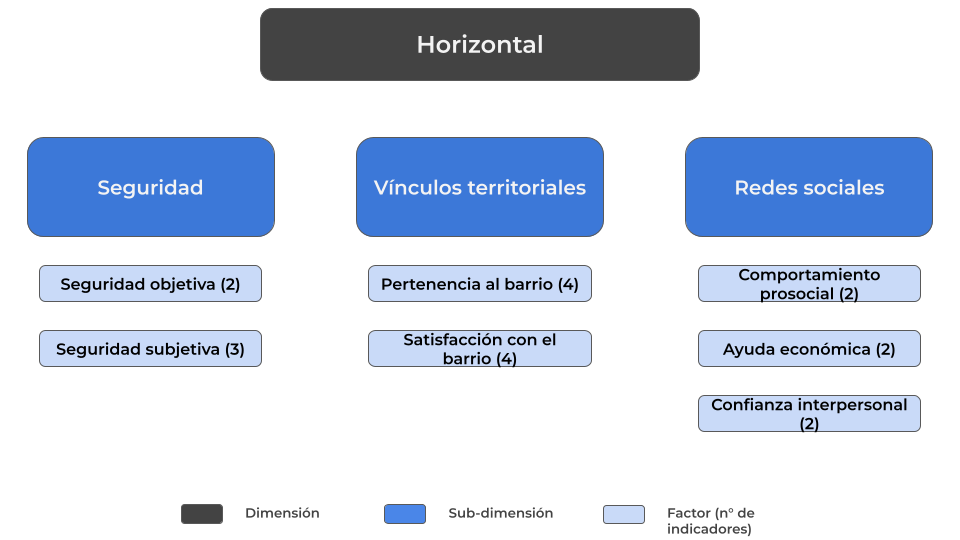
\includegraphics[keepaspectratio]{images/propuesta-nueva.png}}

La propuesta de medición de cohesión social horizontal con ELSOC se basa
en tres subdimensiones: seguridad, vínculos territoriales y redes
sociales.

\begin{itemize}
\item
  Seguridad se mide desde su plano subjetivo, a través de la percepción
  y satisfacción de seguridad con el barrio, y desde su plano objetivo,
  mediante la frecuencia de hechos violentos como asaltos, peleas
  callejeras y tráficos de drogas
\item
  Vínculos territoriales se mide por dos factores; la satisfacción con
  el barrio, tomando en cuenta elementos como la sociabilidad, facilidad
  de hacer amigos, y la cordialidad y colaboración entre vecinos; el
  sentido de pertenencia, el cual aborda elementos identitarios en
  relación al barrio donde vive en encuestado, tales como si es su
  barrio ideal, se identifica con él y si se siente integrado.
\item
  En redes sociales, comportamientos prosociales se mide por la
  asistencia a reuniones públicas y la realización de voluntariado.
  Ayuda económica considera el haber prestado dinero en algún momento a
  alguien y haber ayudado a encontrar trabajo a un tercero. Por último,
  confianza interpersonal considera confianza social generalizada, donde
  se pregunta si se puede o no confiar en la mayoría de las personas, y
  además altruismo social generalizado, el que pregunta si las personas
  generalmente tratan de ayudar a otros o se preocupan de sí mismas
\end{itemize}

\section{2. Aceptación de la diversidad e
interculturalidad}\label{aceptaciuxf3n-de-la-diversidad-e-interculturalidad}

\subsection{Aceptación de la
diversidad}\label{aceptaciuxf3n-de-la-diversidad}

Es la actitud hacia personas de diferentes orígenes y culturas dentro de
una sociedad. Se mide evaluando los siguientes aspectos:

\begin{itemize}
\item
  \textbf{Simpatía hacia migrantes} --- ``¿Cuánto le agradan los
  {[}peruanos/haitianos/venezolanos{]} que viven en Chile?''
\item
  \textbf{Amenaza laboral} --- ``Con la llegada de tantos {[}\ldots{]},
  en Chile está aumentando el desempleo.''
\item
  \textbf{Pérdida de identidad nacional} --- ``Con la llegada de tantos
  {[}\ldots{]}, Chile está perdiendo su identidad.''
\item
  \textbf{Calidad del contacto} --- ``En los últimos 12 meses, cuando
  interactuó con {[}\ldots{]}, ¿cuán amistosa fue la experiencia?''
\item
  \textbf{Políticas más restrictivas} --- ``Chile debería tomar medidas
  más drásticas para impedir el ingreso de inmigrantes al país.''
\end{itemize}

\begin{center}\rule{0.5\linewidth}{0.5pt}\end{center}

\begin{center}\rule{0.5\linewidth}{0.5pt}\end{center}

\begin{center}\rule{0.5\linewidth}{0.5pt}\end{center}

\begin{center}\rule{0.5\linewidth}{0.5pt}\end{center}

\begin{center}\rule{0.5\linewidth}{0.5pt}\end{center}

\begin{center}
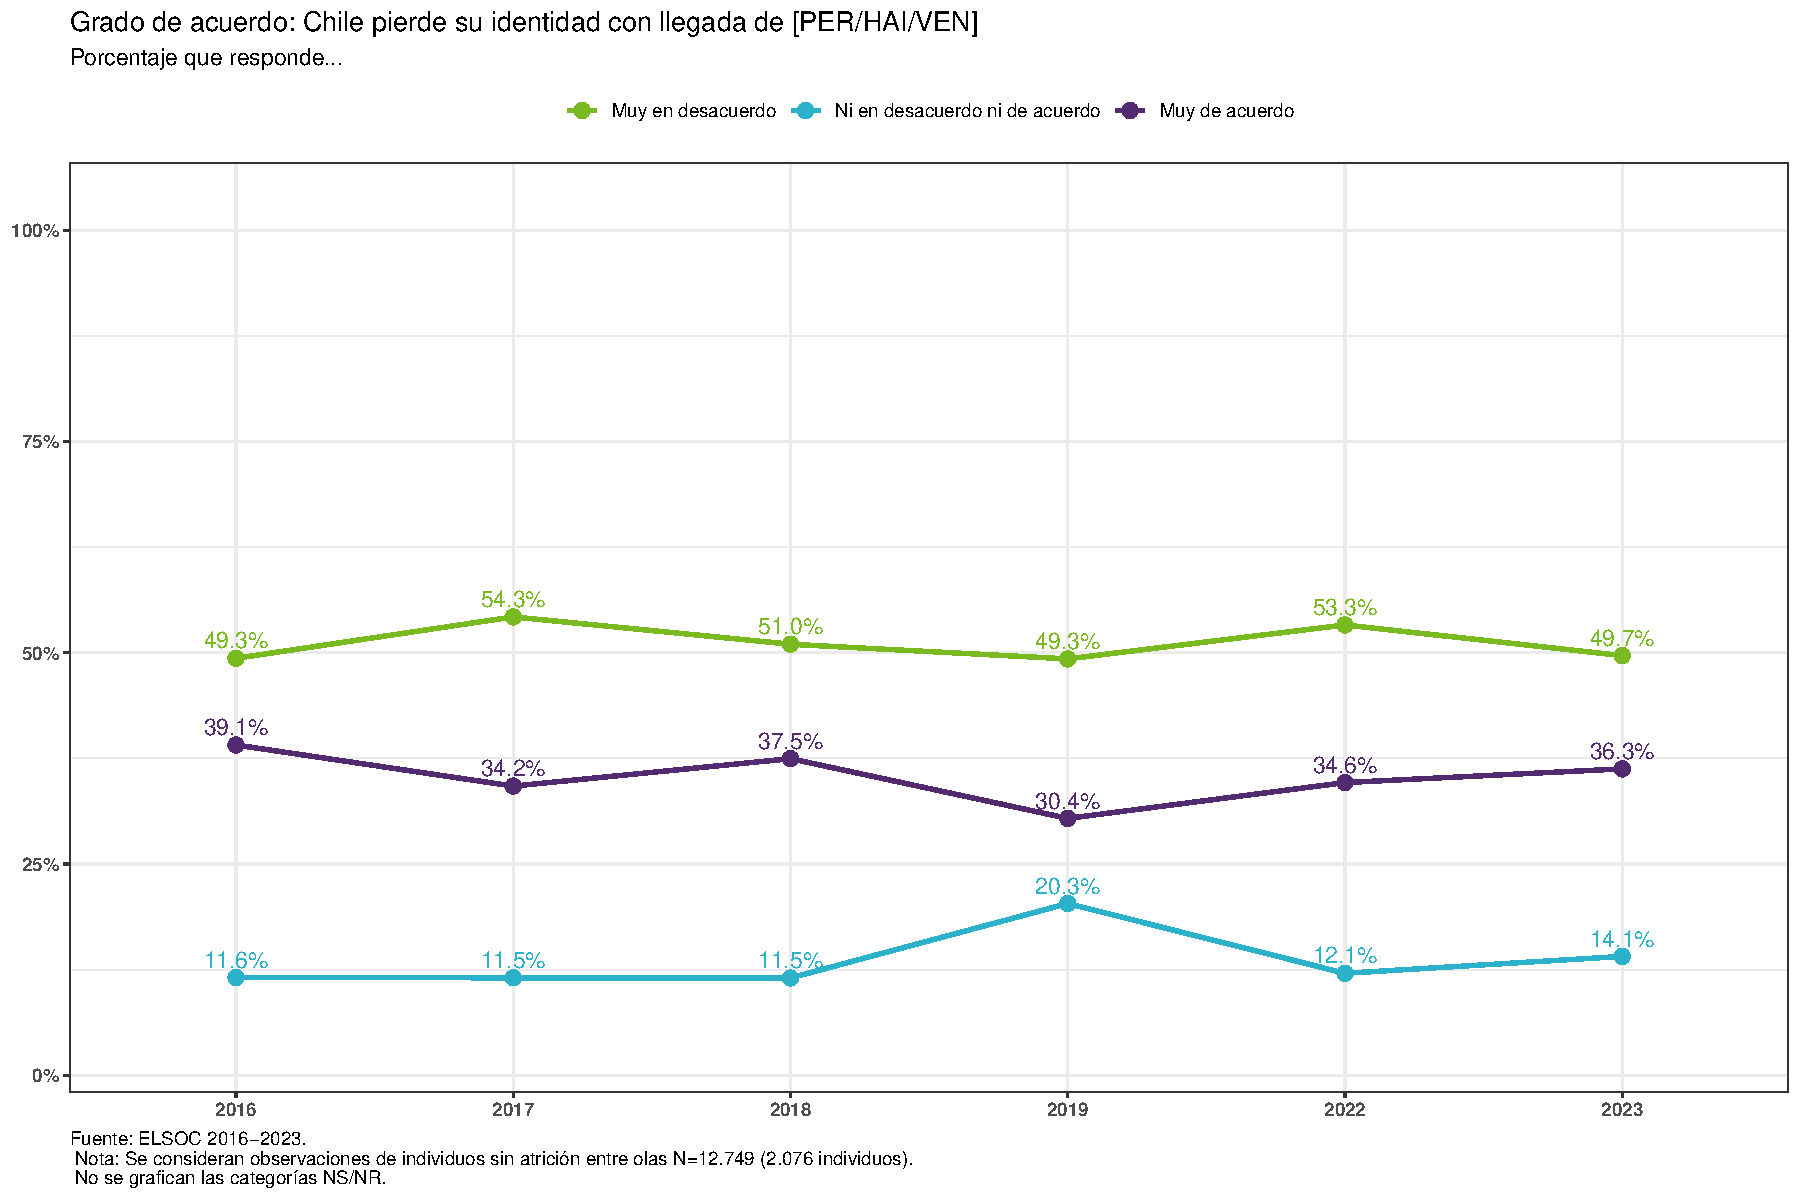
\includegraphics[width=1\linewidth,height=\textheight,keepaspectratio]{cep_2025_files/figure-pdf/unnamed-chunk-2-1.pdf}
\end{center}

\begin{center}\rule{0.5\linewidth}{0.5pt}\end{center}

\begin{center}\rule{0.5\linewidth}{0.5pt}\end{center}

\begin{center}\rule{0.5\linewidth}{0.5pt}\end{center}

\begin{center}\rule{0.5\linewidth}{0.5pt}\end{center}

\begin{center}\rule{0.5\linewidth}{0.5pt}\end{center}

\section{3. Cohesión social horizontal y
migración}\label{cohesiuxf3n-social-horizontal-y-migraciuxf3n}

{\textbf{3.1. Seguridad}}

{\textbf{3.2. Vínculos territoriales}}

{\textbf{3.3. Redes}}

\section{3. Cohesión social horizontal y
migración}\label{cohesiuxf3n-social-horizontal-y-migraciuxf3n-1}

{\textbf{3.1. Seguridad}}

{\textbf{3.2. Vínculos territoriales}}

{\textbf{3.3. Redes}}

\begin{center}\rule{0.5\linewidth}{0.5pt}\end{center}

\begin{center}
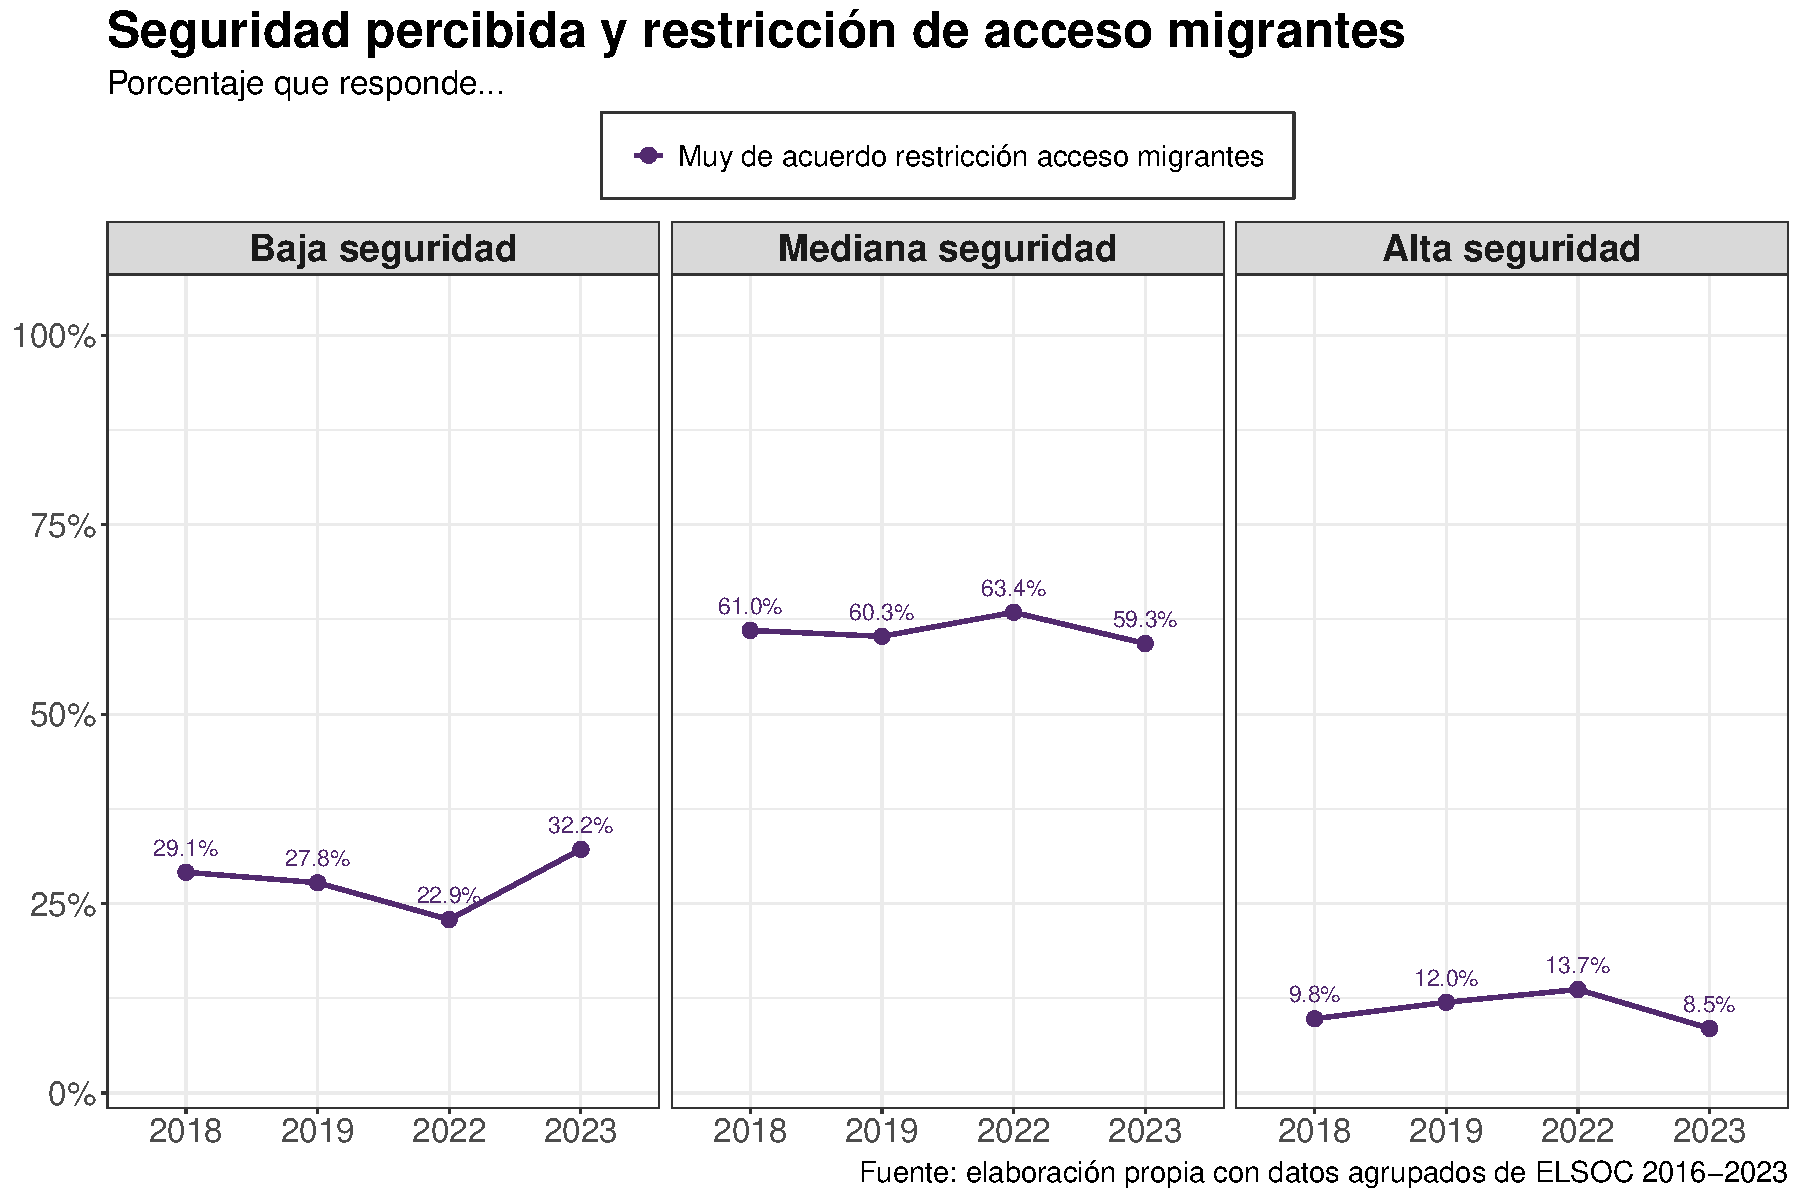
\includegraphics[width=1\linewidth,height=\textheight,keepaspectratio]{cep_2025_files/figure-pdf/unnamed-chunk-4-1.pdf}
\end{center}

\begin{center}\rule{0.5\linewidth}{0.5pt}\end{center}

\begin{center}
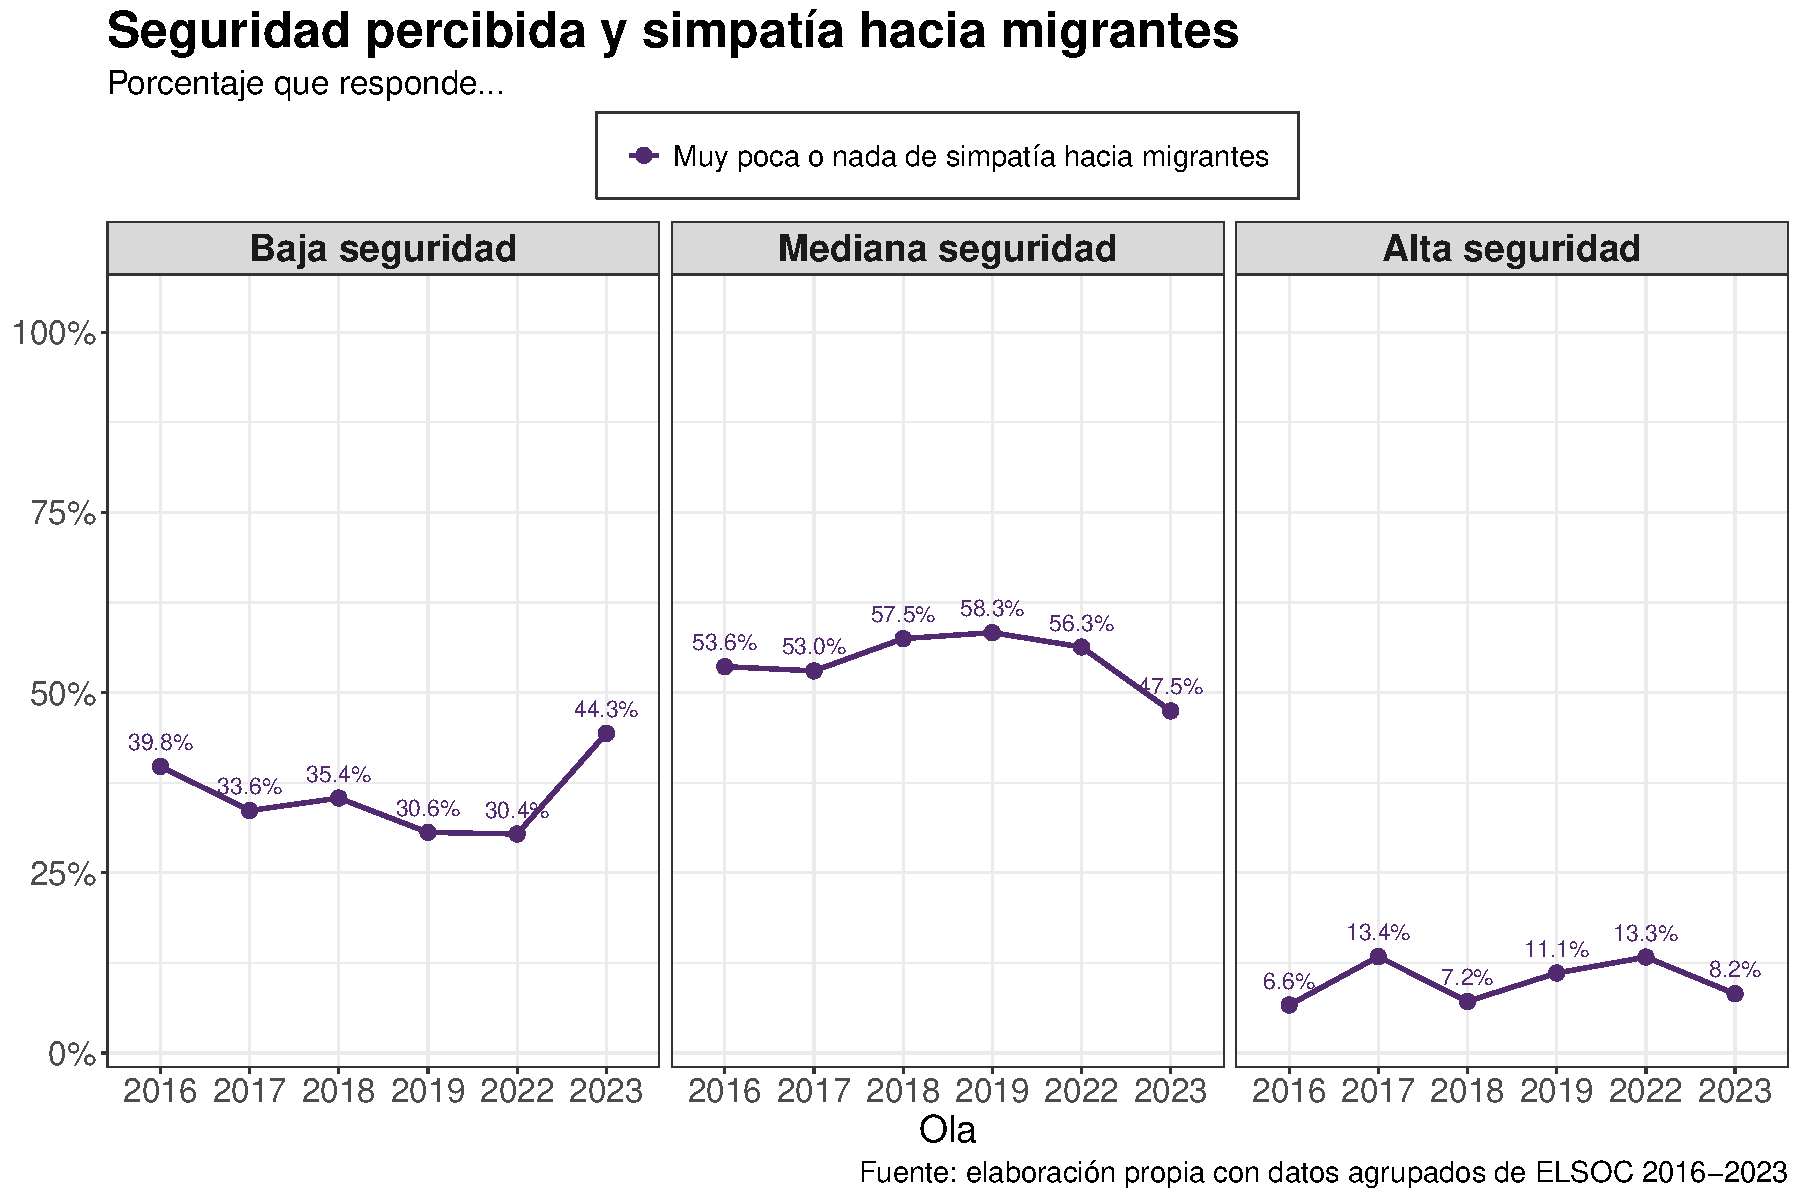
\includegraphics[width=1\linewidth,height=\textheight,keepaspectratio]{cep_2025_files/figure-pdf/unnamed-chunk-5-1.pdf}
\end{center}

\begin{center}\rule{0.5\linewidth}{0.5pt}\end{center}

\begin{center}
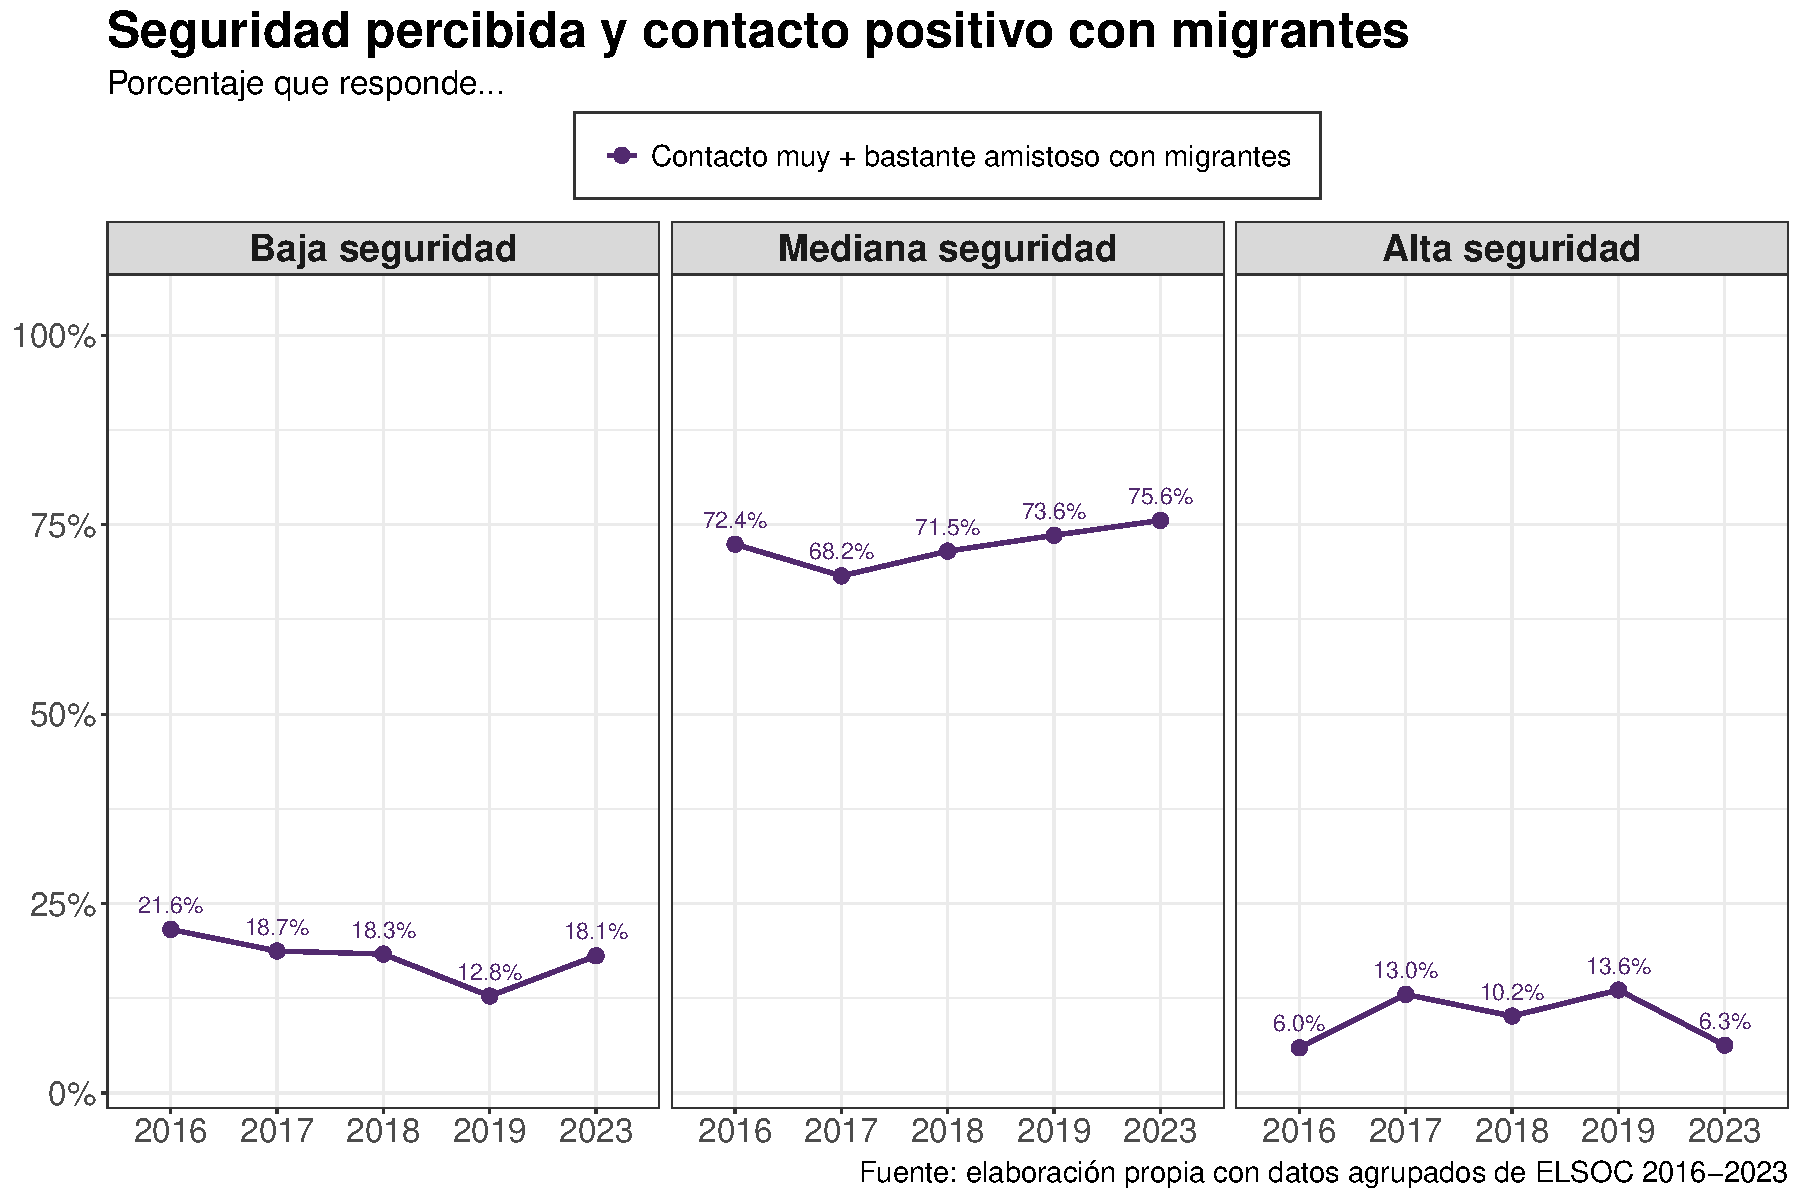
\includegraphics[width=1\linewidth,height=\textheight,keepaspectratio]{cep_2025_files/figure-pdf/unnamed-chunk-6-1.pdf}
\end{center}

\section{3. Cohesión social horizontal y
migración}\label{cohesiuxf3n-social-horizontal-y-migraciuxf3n-2}

{\textbf{3.1. Seguridad}}

{\textbf{3.2. Vínculos territoriales}}

{\textbf{3.3. Redes}}

\begin{center}\rule{0.5\linewidth}{0.5pt}\end{center}

\begin{center}
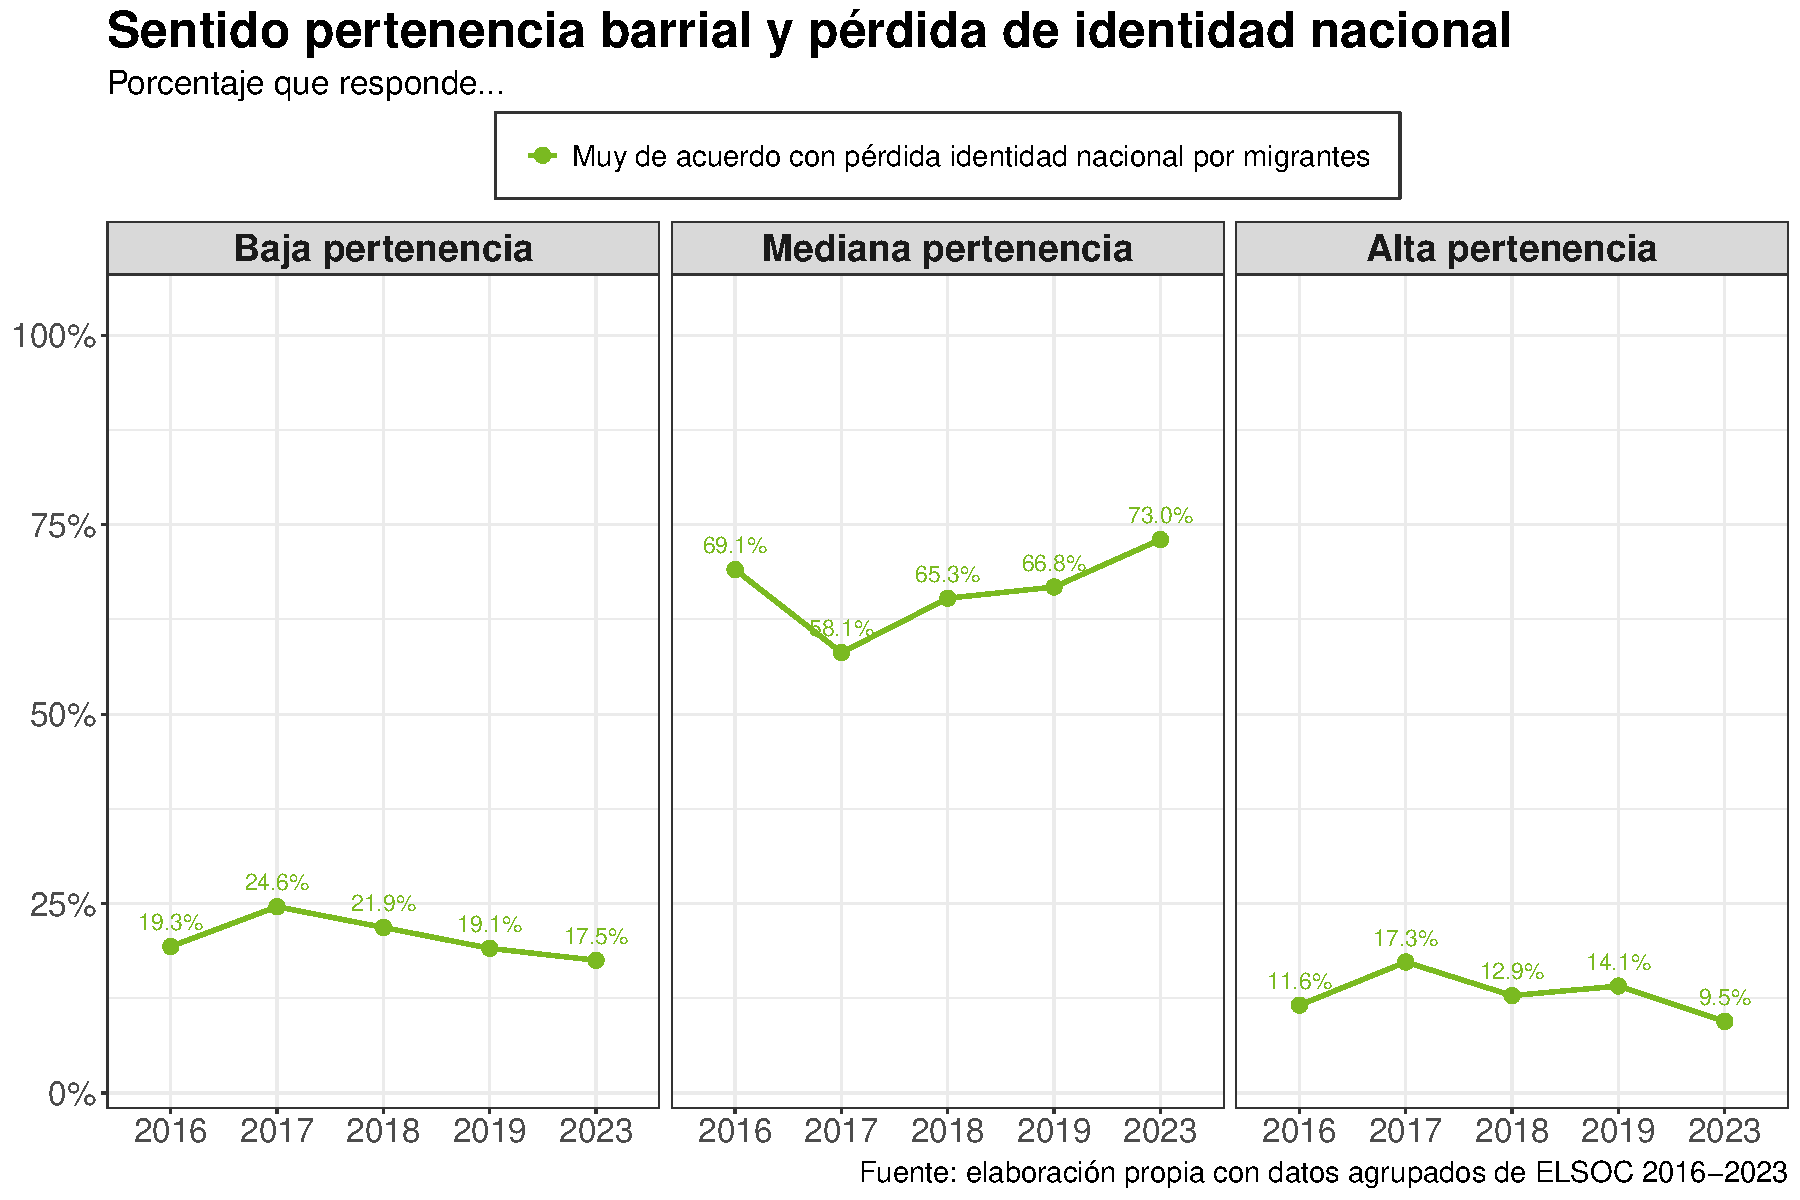
\includegraphics[width=1\linewidth,height=\textheight,keepaspectratio]{cep_2025_files/figure-pdf/unnamed-chunk-7-1.pdf}
\end{center}

\begin{center}\rule{0.5\linewidth}{0.5pt}\end{center}

\begin{center}
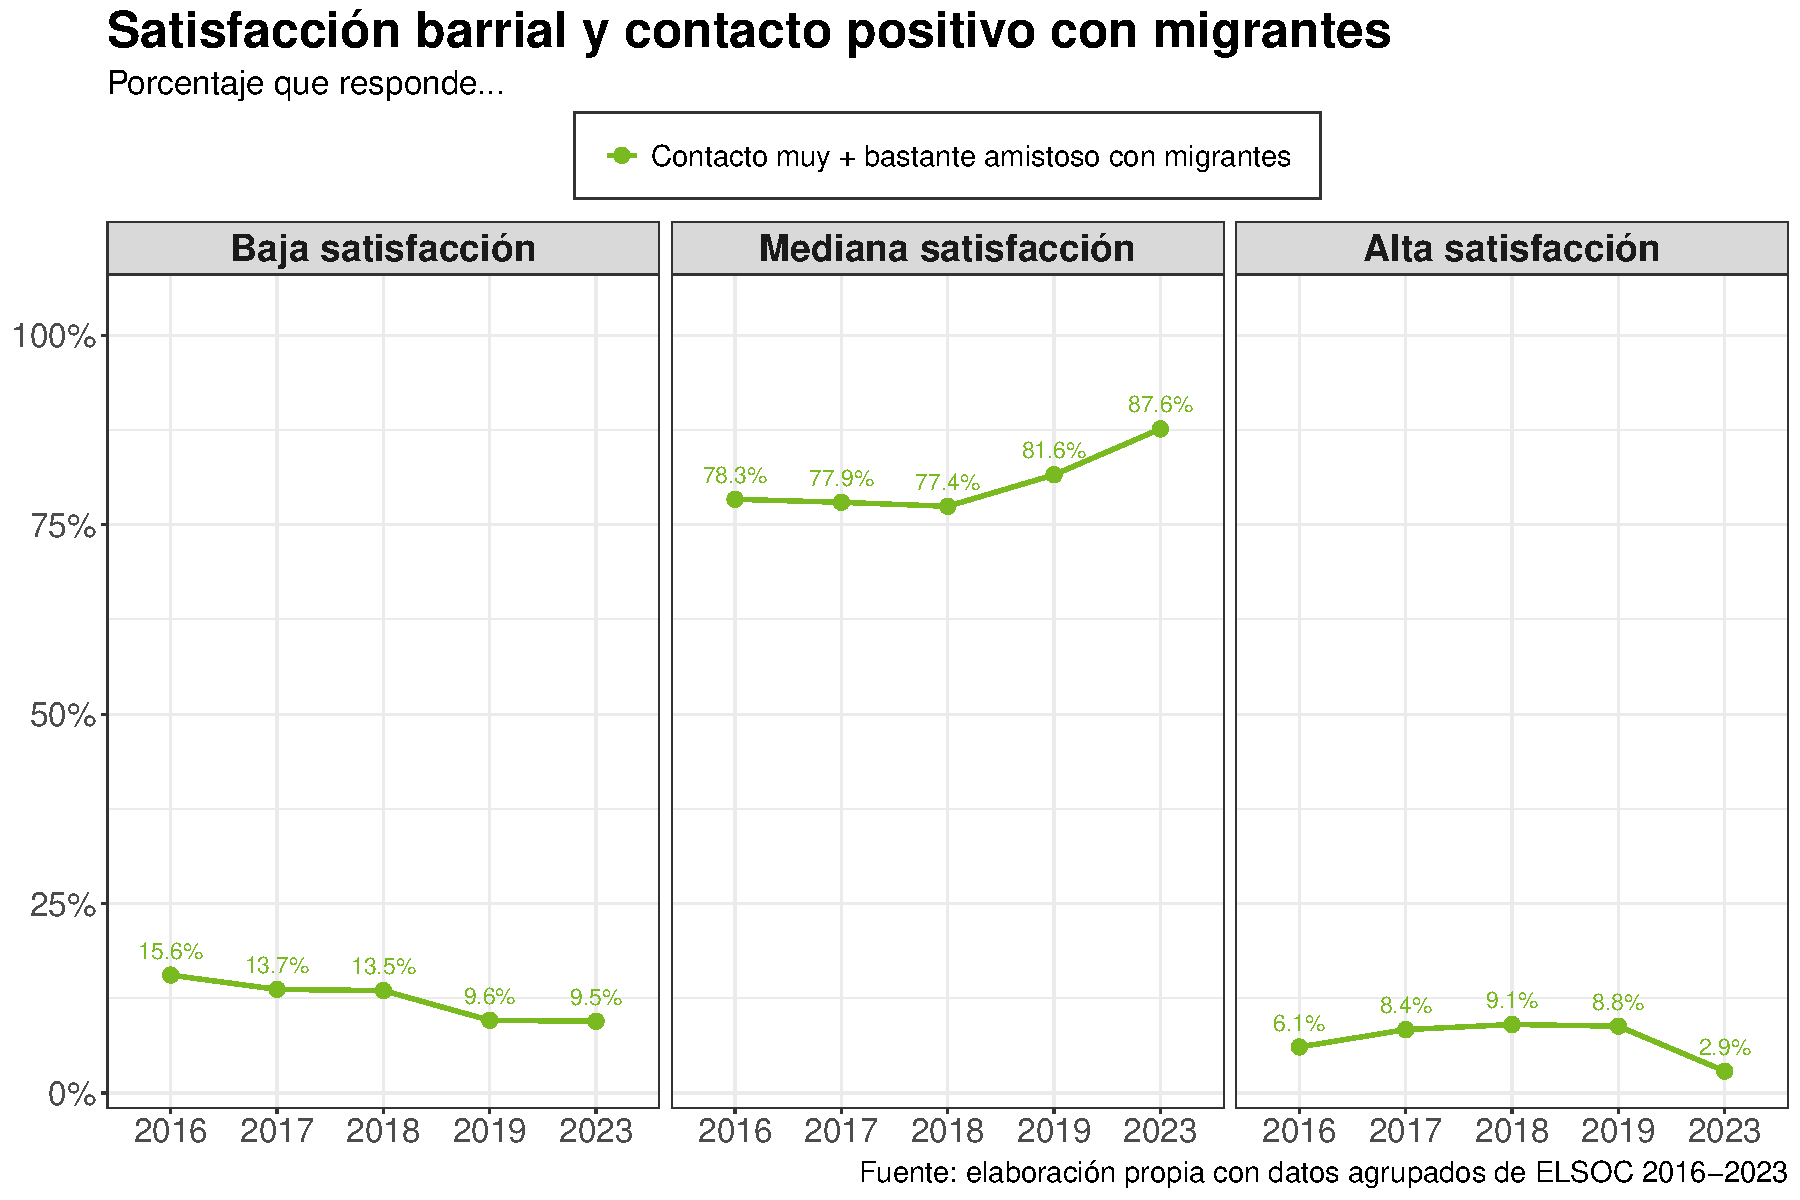
\includegraphics[width=1\linewidth,height=\textheight,keepaspectratio]{cep_2025_files/figure-pdf/unnamed-chunk-8-1.pdf}
\end{center}

\begin{center}\rule{0.5\linewidth}{0.5pt}\end{center}

\begin{center}
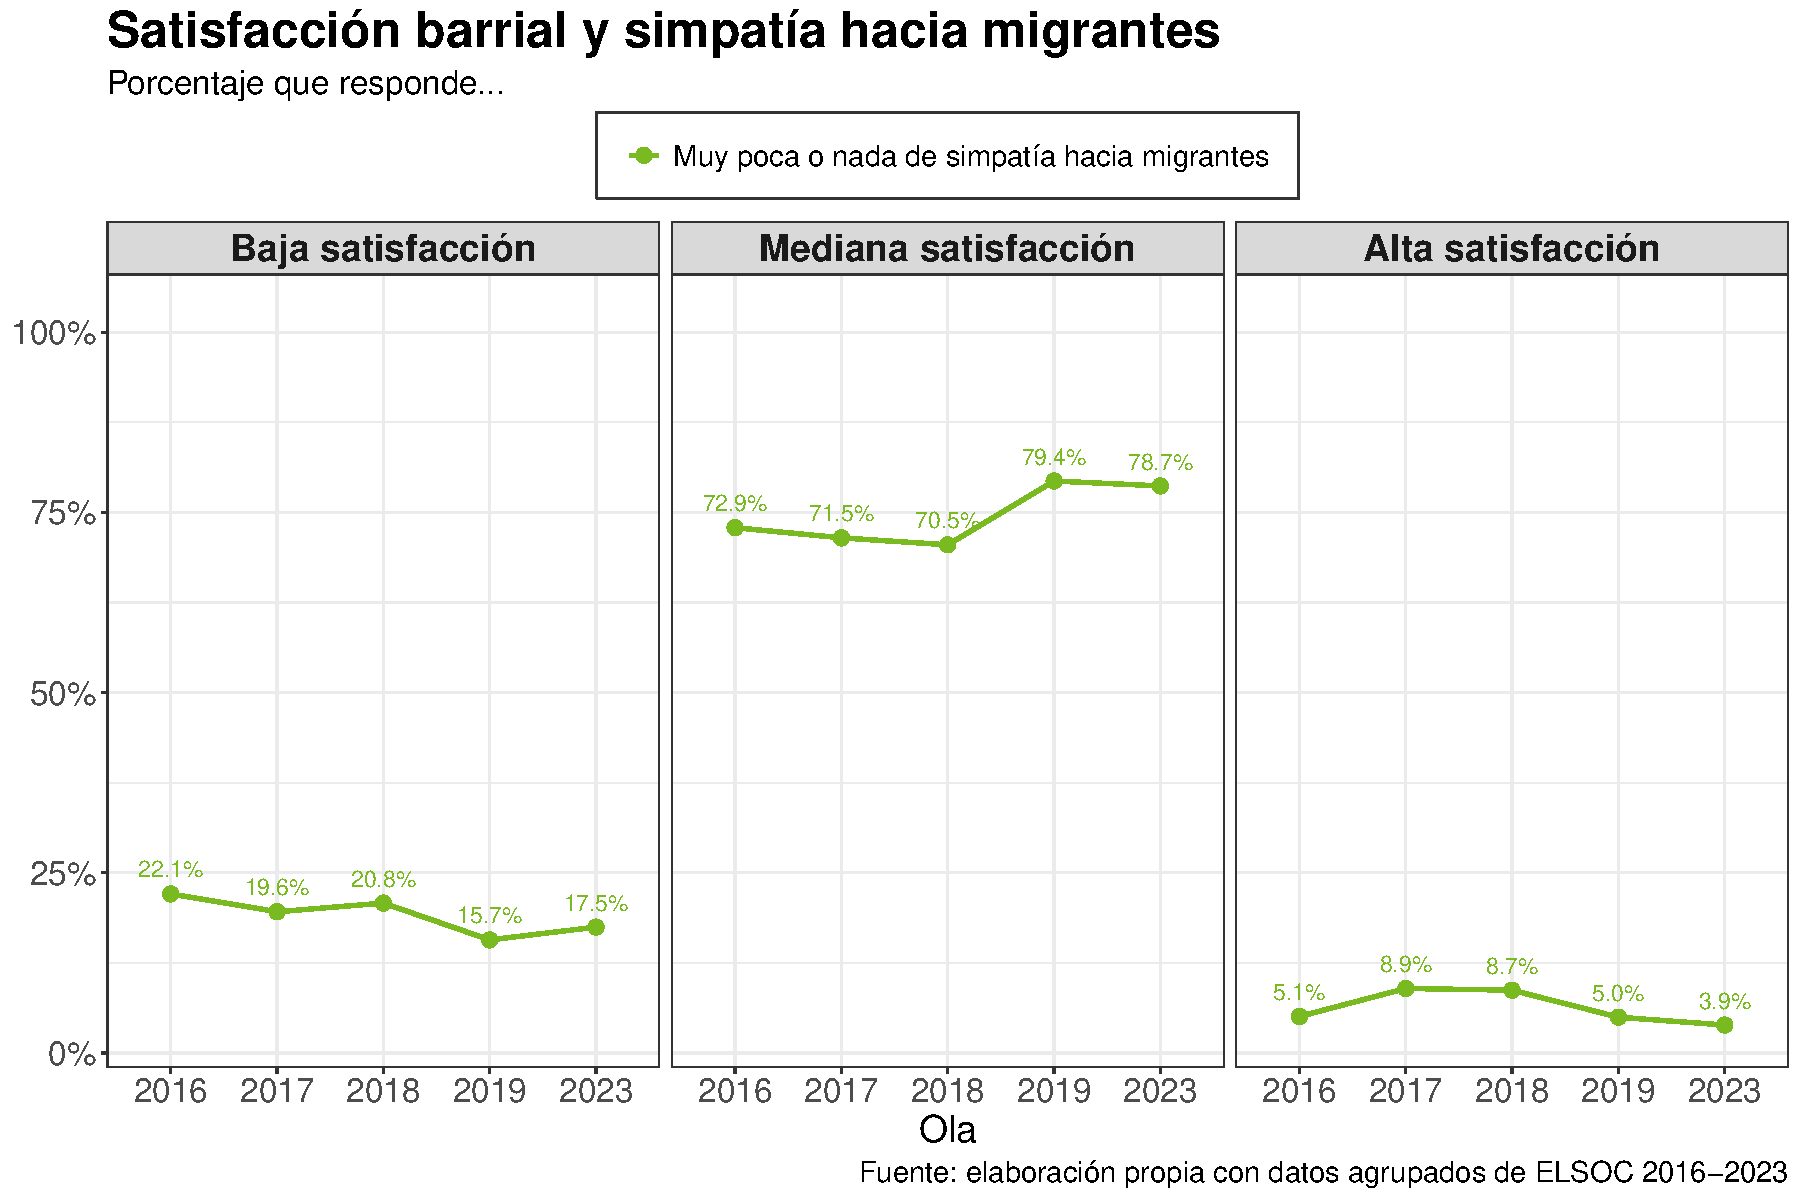
\includegraphics[width=1\linewidth,height=\textheight,keepaspectratio]{cep_2025_files/figure-pdf/unnamed-chunk-9-1.pdf}
\end{center}

\section{3. Cohesión social horizontal y
migración}\label{cohesiuxf3n-social-horizontal-y-migraciuxf3n-3}

{\textbf{3.1. Seguridad}}

{\textbf{3.2. Vínculos territoriales}}

{\textbf{3.3. Redes}}

\begin{center}\rule{0.5\linewidth}{0.5pt}\end{center}

\begin{center}
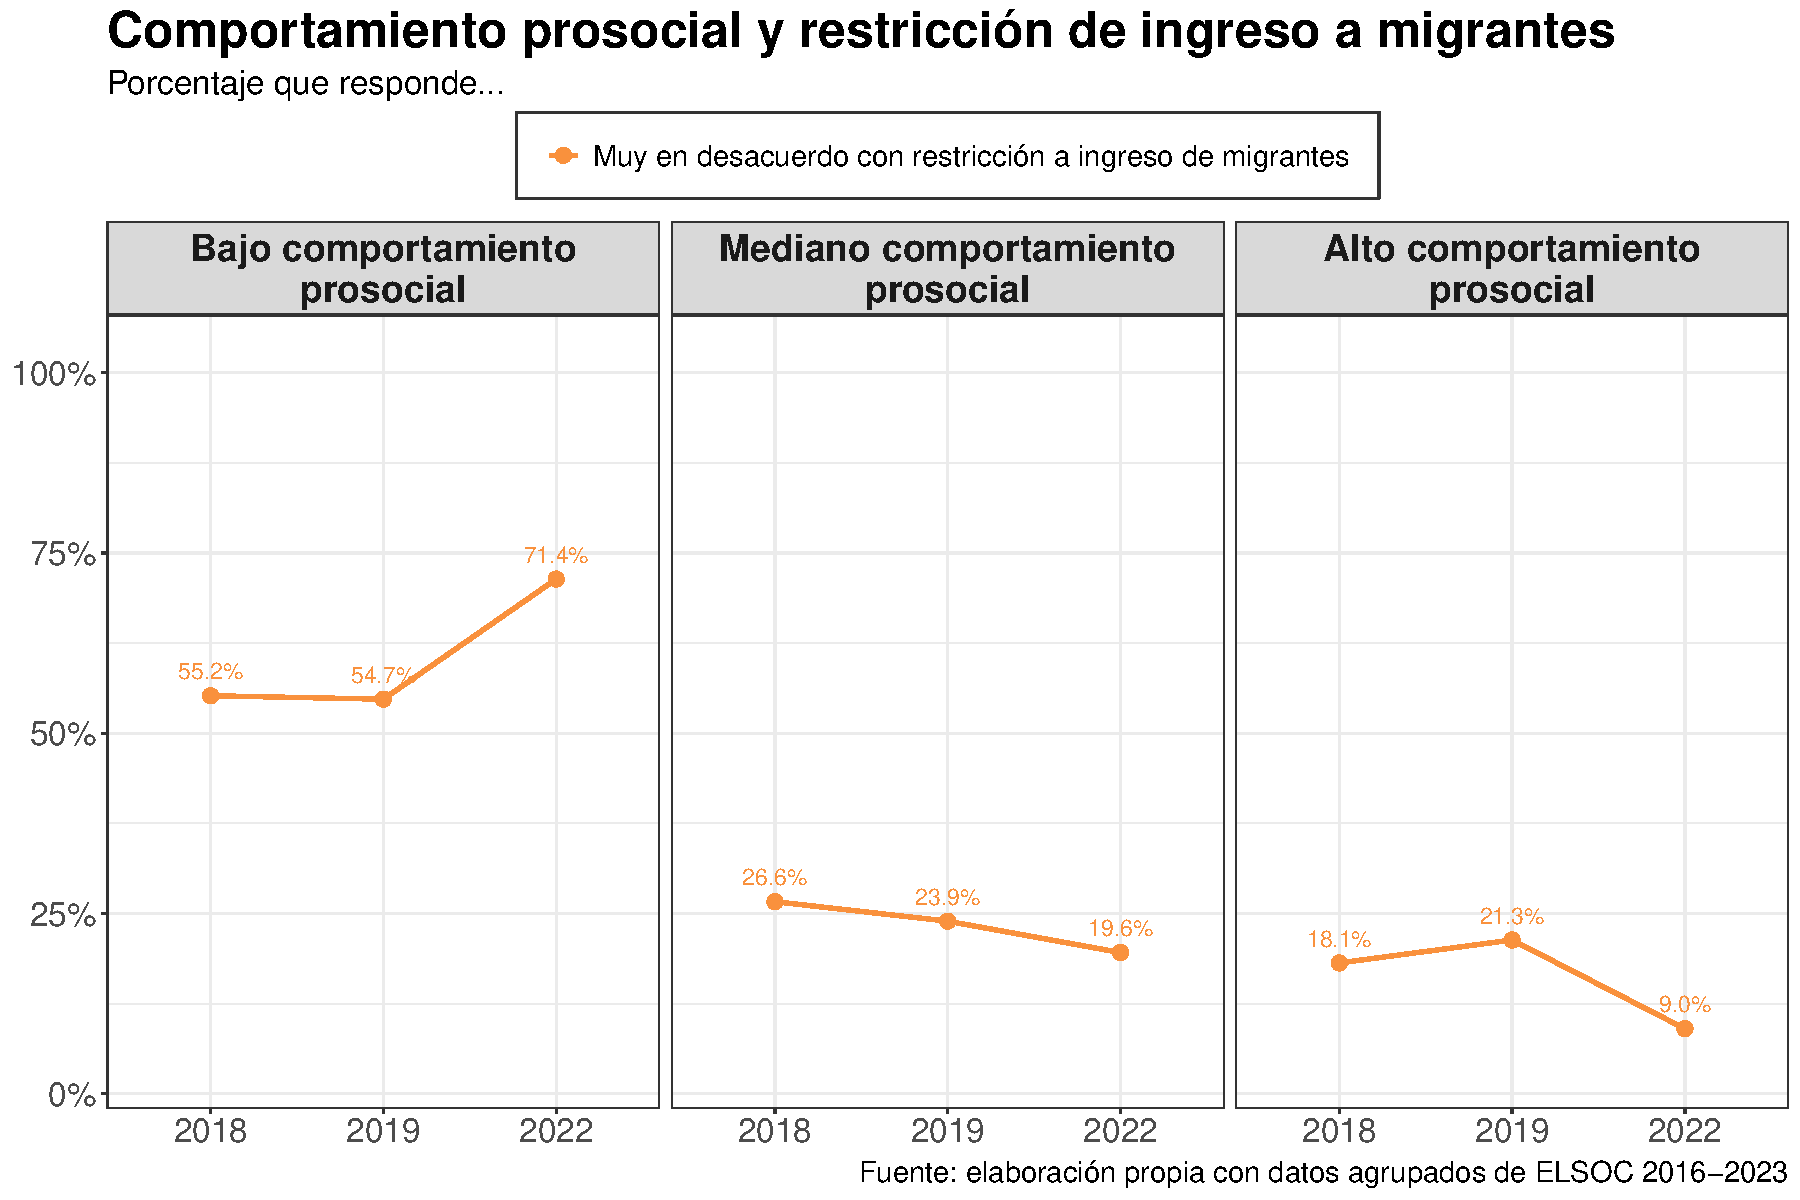
\includegraphics[width=1\linewidth,height=\textheight,keepaspectratio]{cep_2025_files/figure-pdf/unnamed-chunk-10-1.pdf}
\end{center}

\begin{center}\rule{0.5\linewidth}{0.5pt}\end{center}

\begin{center}
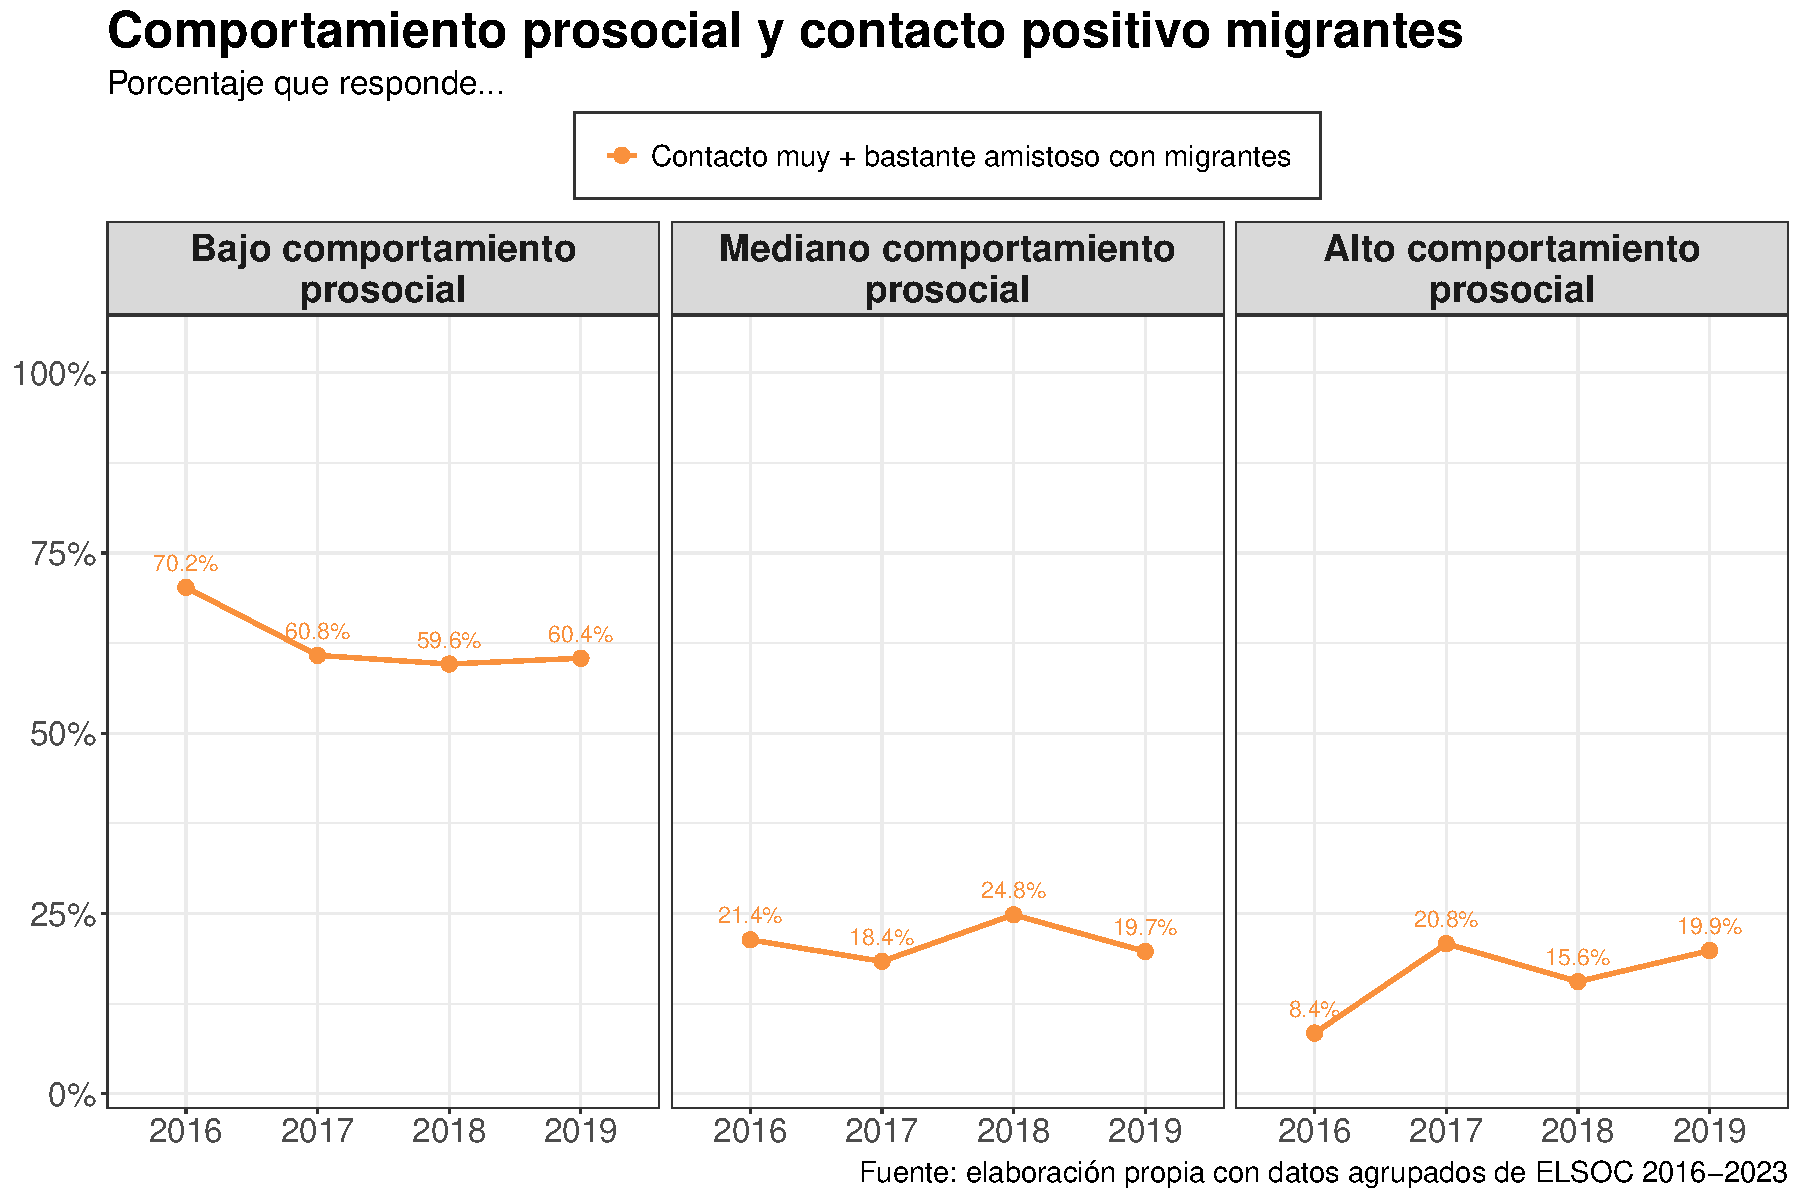
\includegraphics[width=1\linewidth,height=\textheight,keepaspectratio]{cep_2025_files/figure-pdf/unnamed-chunk-11-1.pdf}
\end{center}

\begin{center}\rule{0.5\linewidth}{0.5pt}\end{center}

\begin{center}
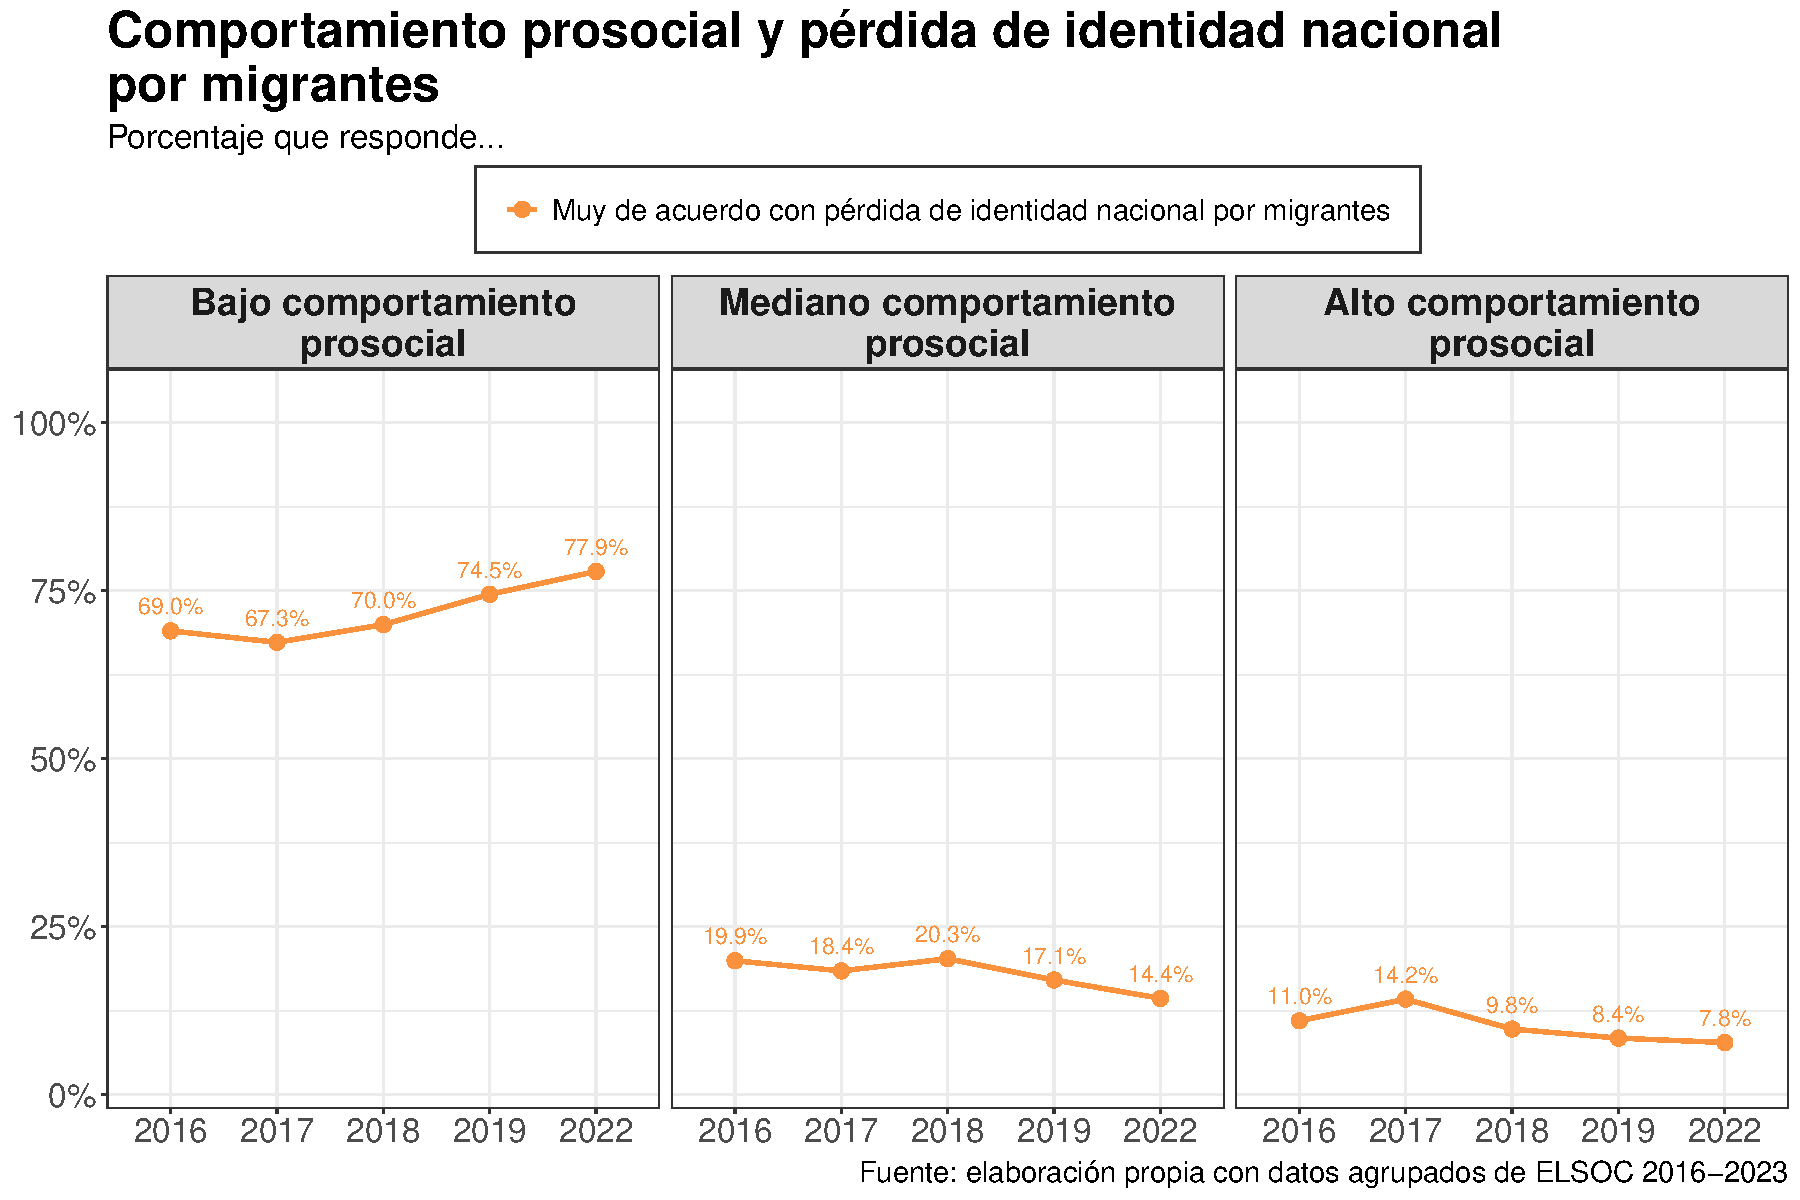
\includegraphics[width=1\linewidth,height=\textheight,keepaspectratio]{cep_2025_files/figure-pdf/unnamed-chunk-12-1.pdf}
\end{center}

\section{4. Conclusiones}\label{conclusiones}

\subsection{Conclusiones}\label{conclusiones-1}

\textbf{1. }:

\textbf{2. }:

\textbf{3. }:

\section{¡Gracias por su atención!}\label{gracias-por-su-atenciuxf3n}

\subsection{Referencias}\label{referencias}

\phantomsection\label{refs}
\begin{CSLReferences}{1}{0}
\bibitem[\citeproctext]{ref-chan_reconsidering_2006}
Chan, J., To, H.-P., \& Chan, E. (2006). Reconsidering {Social
Cohesion}: {Developing} a {Definition} and {Analytical Framework} for
{Empirical Research}. \emph{Social Indicators Research}, \emph{75}(2),
273-302. \url{https://doi.org/10.1007/s11205-005-2118-1}

\bibitem[\citeproctext]{ref-dinesen_trust_2020}
Dinesen, P. T., Schaeffer, M., \& Sønderskov, K. M. (2020). Ethnic
{Diversity} and {Social Trust}: {A Narrative} and {Meta-Analytical
Review}. \emph{Annual Review of Political Science}, \emph{23}(1),
441-465. \url{https://doi.org/10.1146/annurev-polisci-052918-020708}

\bibitem[\citeproctext]{ref-censo_2024}
INE. (2024). Resultados {Fecundidad}, Migraci{ó}n Interna e
Internacional {CENSO} 2024.

\bibitem[\citeproctext]{ref-paolini_intergroup_2014}
Paolini, S., Harwood, J., Rubin, M., Husnu, S., Joyce, N., \& Hewstone,
M. (2014). Positive and Extensive Intergroup Contact in the Past Buffers
against the Disproportionate Impact of Negative Contact in the Present.
\emph{European Journal of Social Psychology}, \emph{44}(6), 548-562.
\url{https://doi.org/10.1002/ejsp.2029}

\bibitem[\citeproctext]{ref-reibold_trust_2025}
Reibold, K., Bachvarova, M., \& Lenard, P. T. (2025). Introduction:
Trust, Social Cohesion, and Integration. \emph{Critical Review of
International Social and Political Philosophy}, 1-18.
\url{https://doi.org/10.1080/13698230.2025.2528379}

\end{CSLReferences}




\end{document}
